% Slide bảo vệ đồ án Lập trình mạng, dựng theo template ~/Downloads/main.tex (pdfLaTeX, tiếng Việt T5).
% Biên dịch: cd slides && latexmk -pdf main.tex
\documentclass[aspectratio=169,10pt]{beamer}

% =================================================
% TIẾNG VIỆT
% =================================================
\usepackage[T5]{fontenc}
\usepackage[utf8]{inputenc}
\usepackage[vietnamese]{babel}

% =================================================
% THƯ VIỆN
% =================================================
\usepackage{graphicx}
\usepackage{tikz}
\usetikzlibrary{arrows.meta,positioning,calc}
\usepackage{booktabs}
\usepackage{tabularx}
\usepackage{amsmath,amssymb}
\usepackage{url}
\graphicspath{{../docs/figures/}{../experiments/results/}}

% =================================================
% GIAO DIỆN
% =================================================
\usetheme{Madrid}

\definecolor{MainBlue}{HTML}{153B60}
\definecolor{Accent}{HTML}{087E8B}
\definecolor{CodeBG}{HTML}{F3F5F7}
\definecolor{Good}{HTML}{157A3A}
\definecolor{Bad}{HTML}{B42318}
\definecolor{U0}{HTML}{2A78D6}

\setbeamercolor{structure}{fg=MainBlue}
\setbeamercolor{frametitle}{bg=MainBlue,fg=white}
\setbeamercolor{title}{bg=MainBlue,fg=white}
\setbeamercolor{block title}{bg=MainBlue!12,fg=MainBlue}
\setbeamercolor{block body}{bg=MainBlue!4}
\setbeamercolor{alerted text}{fg=Bad}

\setbeamertemplate{navigation symbols}{}
\setbeamersize{text margin left=7mm,text margin right=7mm}
\setbeamertemplate{itemize items}[circle]
\setlength{\parskip}{3pt}

\tikzset{
  box/.style={draw=MainBlue!70,fill=MainBlue!7,rounded corners=3pt,align=center,text width=2.5cm,minimum height=8mm,font=\small},
  arr/.style={-{Stealth[length=2mm]},thick,draw=Accent},
}

\newcommand{\good}[1]{\textcolor{Good}{\textbf{#1}}}
\newcommand{\hl}[1]{\textcolor{MainBlue}{\textbf{#1}}}
\newcommand{\SE}{\widehat{SE}}

% Bố cục báo cáo: nền trắng, tiêu đề xanh, bỏ hộp và bóng đổ (giống template).
\setbeamercolor{normal text}{fg=black!90,bg=white}
\setbeamercolor{frametitle}{fg=MainBlue,bg=white}
\setbeamerfont{frametitle}{size=\large,series=\bfseries}
\setbeamertemplate{frametitle}{%
  \vspace{2mm}%
  \insertframetitle\par
  \vspace{1mm}%
  {\color{MainBlue!35}\hrule height 0.4pt}%
  \vspace{1mm}%
}
\setbeamerfont{block title}{size=\small,series=\bfseries}
\setbeamertemplate{block begin}{%
  \vskip0.7ex
  {\usebeamerfont{block title}\color{MainBlue}\insertblocktitle\par}%
  \vskip0.3ex
  \usebeamerfont{block body}%
}
\setbeamertemplate{block end}{\vskip0.5ex}
\setbeamertemplate{enumerate items}[default]
\setbeamercolor{itemize item}{fg=MainBlue}
\setbeamercolor{itemize subitem}{fg=MainBlue}
\setbeamerfont{footline}{size=\tiny}
\setbeamertemplate{footline}{%
  \hfill{\color{black!50}\insertframenumber/\inserttotalframenumber}\hspace{5mm}\vspace{2mm}%
}

% Khung mã giả (không dùng listings vì listings không hỗ trợ tiếng Việt dưới pdfLaTeX)
\newenvironment{pseudo}{%
  \begin{beamercolorbox}[sep=2mm,rounded=true]{block body}\scriptsize\begin{tabbing}
  \hspace{4mm}\=\hspace{4mm}\=\hspace{4mm}\=\hspace{4mm}\=\kill}%
  {\end{tabbing}\end{beamercolorbox}}
\newcommand{\kw}[1]{\textbf{\textcolor{MainBlue}{#1}}}
\newcommand{\cm}[1]{\textcolor{gray}{\ // #1}}

\title{Cấp phát tài nguyên cho mạng nhiều UAV làm trạm gốc có ưu tiên người dùng}
\date{}

\begin{document}

% =================================================
% SLIDE 1. TRANG BÌA
% =================================================
\begin{frame}[plain]
\begin{tikzpicture}[remember picture,overlay,x=\paperwidth,y=\paperheight]
\begin{scope}[shift={(current page.south west)}]
\fill[white] (0,0) rectangle (1,1);
\node[anchor=north,align=center,text=MainBlue,text width=0.90\paperwidth,font=\fontsize{10}{14}\selectfont\bfseries] at (0.5,0.93) {TRƯỜNG ĐẠI HỌC BÁCH KHOA -- ĐẠI HỌC ĐÀ NẴNG\\ KHOA ĐIỆN TỬ VÀ TRÍ TUỆ NHÂN TẠO};
\draw[MainBlue!35,line width=0.5pt] (0.12,0.79)--(0.88,0.79);
\node[text=MainBlue,font=\fontsize{11}{14}\selectfont] at (0.5,0.71) {LẬP TRÌNH MẠNG -- ĐỒ ÁN CUỐI KỲ};
\node[align=center,text=MainBlue,text width=0.92\paperwidth,font=\fontsize{21}{27}\selectfont\bfseries] at (0.5,0.53) {Cấp phát tài nguyên cho mạng nhiều UAV\\làm trạm gốc có ưu tiên người dùng};
\node[align=center,text=black!70,text width=0.85\paperwidth,font=\fontsize{11}{14}\selectfont] at (0.5,0.37) {Heuristic cải tiến \textbf{calib-ifair}, kiểm chứng ở mức gói tin bằng NS-3 LTE};
\node[anchor=west,align=left,text=black!85,text width=0.80\paperwidth,font=\fontsize{11}{17}\selectfont] at (0.13,0.17) {\textbf{GVHD:} \ldots\\[2mm]\textbf{SVTH:} \ldots};
\end{scope}
\end{tikzpicture}
\mbox{}
\end{frame}

% =================================================
% SLIDE 2. NỘI DUNG
% =================================================
\begin{frame}{Nội dung trình bày}
\begin{columns}[T,onlytextwidth]
\begin{column}{0.48\textwidth}
  \begin{block}{1. Bài toán}
    \begin{itemize}
      \item Kịch bản UAV làm trạm gốc.
      \item Ba nhóm người dùng.
      \item Mô hình kênh, SINR, tốc độ.
      \item Phát biểu bài toán, bài toán tối ưu.
    \end{itemize}
  \end{block}
  \begin{block}{2. Heuristic calib-ifair}
    \begin{itemize}
      \item Liên kết và SINR có nhiễu.
      \item Chia băng ifair, ví dụ số.
      \item Di chuyển calib.
      \item Mã giả, độ phức tạp, áp ở tầng MAC.
    \end{itemize}
  \end{block}
\end{column}
\begin{column}{0.48\textwidth}
  \begin{block}{3. Kiểm chứng bằng NS-3 LTE}
    \begin{itemize}
      \item Ba tầng kiểm chứng.
      \item Baseline, cài đặt, thông số thí nghiệm.
      \item Kết quả theo từng nhóm.
      \item Lợi ích đến từ đâu.
    \end{itemize}
  \end{block}
  \begin{block}{4. Hệ thống và tổng kết}
    \begin{itemize}
      \item Dashboard web, Gazebo.
      \item Đánh đổi, hạn chế.
      \item Kết luận.
    \end{itemize}
  \end{block}
\end{column}
\end{columns}
\end{frame}

% =================================================
% SLIDE 3. BỐI CẢNH
% =================================================
\begin{frame}{Bối cảnh và vấn đề}
\begin{columns}[T,onlytextwidth]
\begin{column}{0.53\textwidth}
  \begin{block}{Bối cảnh}
    \small
    Thiên tai, sự kiện đông người: trạm gốc mặt đất hỏng hoặc quá tải.
    UAV mang trạm gốc LTE (UAV-BS) bay tới vùng cần phủ sóng trong vài phút.
  \end{block}
  \begin{block}{Ba khó khăn}
    \small
    \begin{itemize}
      \item Vị trí UAV quyết định chất lượng kênh.
      \item Các UAV dùng chung băng tần nên \alert{nhiễu nhau}.
      \item Người dùng \hl{không quan trọng như nhau}: đội cứu hộ, y tế cần kết nối chắc hơn người dân.
    \end{itemize}
  \end{block}
  \begin{block}{Khoảng trống}
    \small
    Các bài báo thường tính bằng công thức Shannon. Kết quả khi đo ở mức gói tin trên mạng LTE thật thì sao?
  \end{block}
\end{column}
\begin{column}{0.43\textwidth}
  \centering
  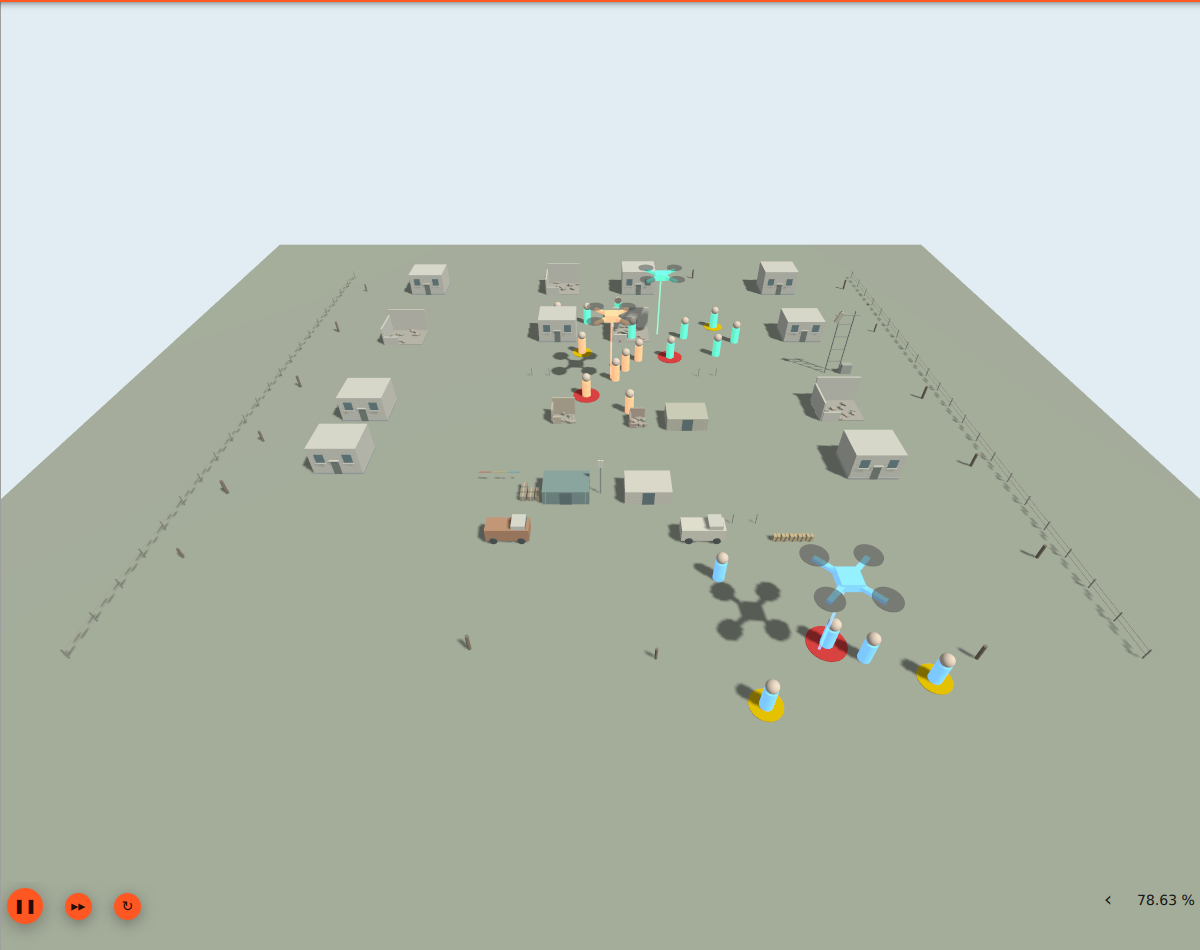
\includegraphics[width=\linewidth]{gazebo.png}

  {\scriptsize Kịch bản trên bãi thảm họa (Gazebo): người mặc áo màu UAV phục vụ, vòng đỏ là user critical.}
\end{column}
\end{columns}
\end{frame}

% =================================================
% SLIDE 4. KỊCH BẢN
% =================================================
\begin{frame}{Kịch bản và ba nhóm người dùng}
\begin{columns}[T,onlytextwidth]
\begin{column}{0.58\textwidth}
  \centering
  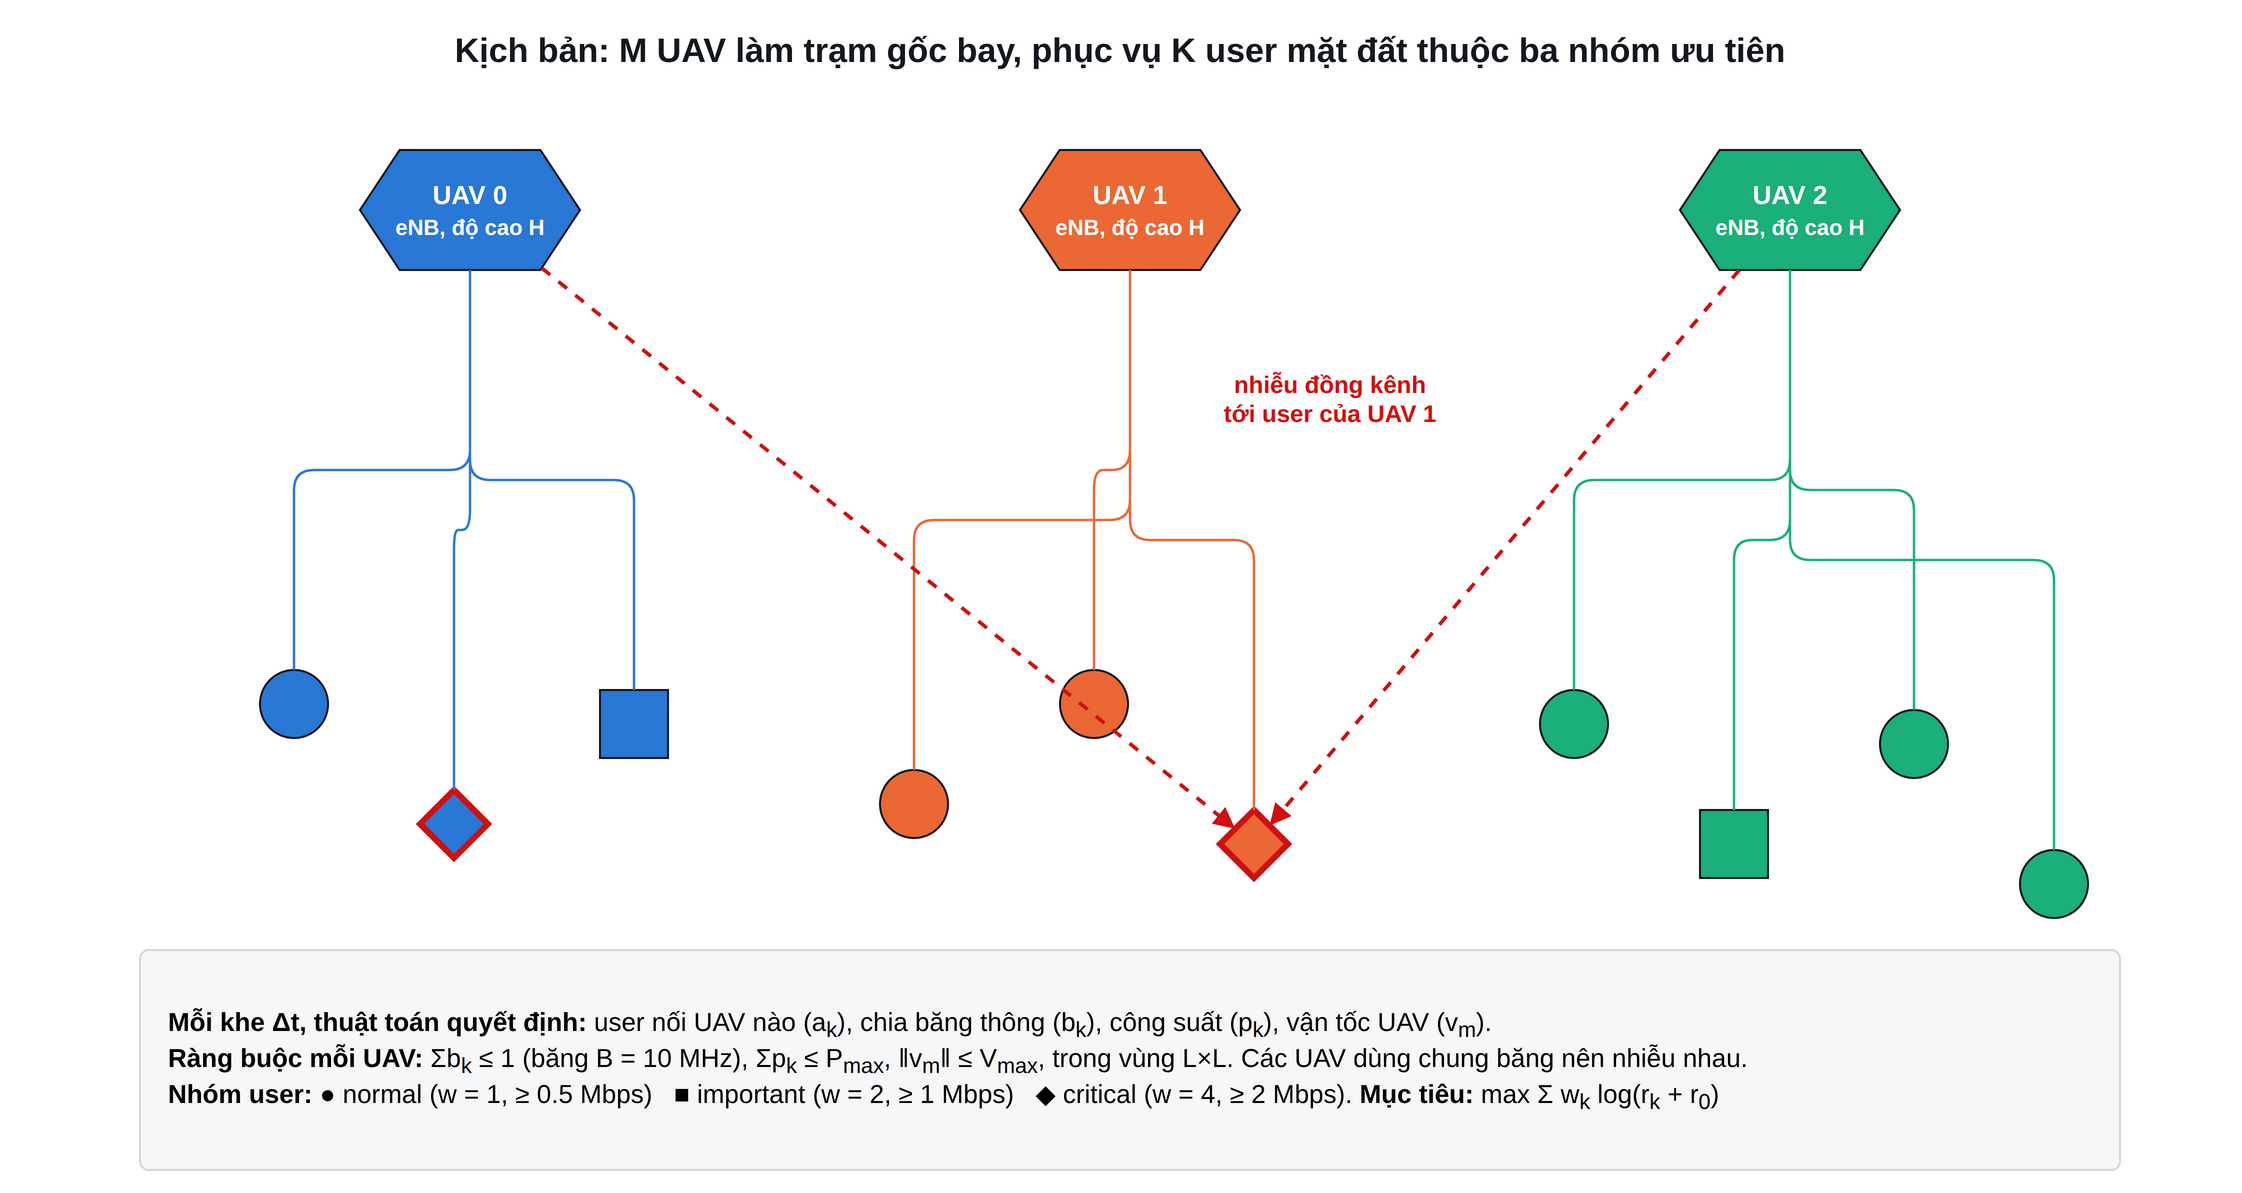
\includegraphics[width=\linewidth]{kich_ban.png}
\end{column}
\begin{column}{0.38\textwidth}
  \small
  \begin{tabularx}{\linewidth}{@{}lccc@{}}
    \toprule
    \textbf{Nhóm} & $w_c$ & $r_{\min,c}$ & \textbf{Tỷ lệ}\\
    \midrule
    normal & 1 & 0.5 Mbps & 60\%\\
    important & 2 & 1 Mbps & 25\%\\
    \textcolor{Bad}{critical} & 4 & 2 Mbps & 15\%\\
    \bottomrule
  \end{tabularx}

  \begin{block}{Quyết định mỗi khe $\Delta t$}
    \scriptsize
    \begin{itemize}
      \item $a_k$: user $k$ nối UAV nào.
      \item $b_k$: phần băng thông cho user $k$.
      \item $p_k = b_k P_{\max}$: công suất theo băng.
      \item $q_m$: vị trí UAV $m$ (qua vận tốc $v_m$).
    \end{itemize}
  \end{block}
  \scriptsize 3 UAV, 20 user, vùng $1\times1$ km, độ cao 100 m, $B = 10$ MHz.
\end{column}
\end{columns}
\end{frame}

% =================================================
% PHÁT BIỂU BÀI TOÁN
% =================================================
\begin{frame}{Phát biểu bài toán}
\begin{columns}[T,onlytextwidth]
\begin{column}{0.48\textwidth}
  \begin{block}{Đầu vào}
    \small
    \begin{itemize}
      \item Vị trí $K$ user và nhóm của từng user (normal / important / critical).
      \item Vị trí hiện tại của $M$ UAV, độ cao cố định $H$.
      \item Tham số vô tuyến: băng $B$, công suất $P_{\max}$, nhiễu $N_0$, môi trường kênh.
      \item Lưu lượng gửi tới mỗi user $\lambda$ (Mbps).
    \end{itemize}
  \end{block}
  \begin{block}{Đầu ra (mỗi khe $\Delta t$)}
    \small
    Liên kết $a_k$, phần băng thông $b_k$, công suất $p_k$, vận tốc $v_m$ của từng UAV.
  \end{block}
\end{column}
\begin{column}{0.48\textwidth}
  \begin{block}{Mục tiêu}
    \small
    Ưu tiên user critical, rồi important, \textbf{nhưng không bỏ rơi} user normal; giữ hiệu quả tổng ở mức chấp nhận được.
  \end{block}
  \begin{block}{Giả thiết}
    \small
    \begin{itemize}
      \item Đường xuống; các UAV dùng chung băng (nhiễu đồng kênh).
      \item Độ cao cố định; kênh dùng suy hao trung bình Al-Hourani.
      \item Mỗi user một hàng đợi tại UAV, bộ đệm 1 MiB.
      \item Thuật toán biết vị trí và nhóm của user.
    \end{itemize}
  \end{block}
  \begin{block}{Câu hỏi kiểm chứng}
    \small
    Kết quả có đứng vững khi đo ở mức gói tin trên NS-3 LTE không?
  \end{block}
\end{column}
\end{columns}
\end{frame}

% =================================================
% SLIDE 5. MÔ HÌNH KÊNH
% =================================================
\begin{frame}{Mô hình kênh, SINR và tốc độ}
\begin{block}{Kênh không -- đất Al-Hourani (đô thị)}
\vspace{-3mm}
\[
P_{\text{LoS}}(\theta) = \frac{1}{1 + a\,e^{-b(\theta - a)}},\qquad
\overline{PL}_{mk} = 20\log_{10}\frac{4\pi f_c d_{mk}}{c} + P_{\text{LoS}}\,\eta_{\text{LoS}} + (1-P_{\text{LoS}})\,\eta_{\text{NLoS}}
\]
\end{block}
\begin{block}{SINR có nhiễu đồng kênh}
\vspace{-3mm}
\[
\mathrm{SINR}_k = \frac{\dfrac{p_k}{b_k B}\, g_{a_k k}(q_{a_k})}{\displaystyle\sum_{j \ne a_k} \frac{P_j}{B}\, g_{jk}(q_j) + N_0},
\qquad g_{mk} = 10^{-\overline{PL}_{mk}/10}
\]
\end{block}
\begin{columns}[T,onlytextwidth]
\begin{column}{0.48\textwidth}
  \begin{block}{Tốc độ theo bài báo (Shannon)}
    \vspace{-2mm}
    \[ r_k = b_k\, B \log_2(1 + \mathrm{SINR}_k) \]
  \end{block}
\end{column}
\begin{column}{0.48\textwidth}
  \begin{block}{Tốc độ LTE hiệu chỉnh từ NS-3}
    \vspace{-2mm}
    \[ \SE_k = \min\big(0.401\log_2(1+\mathrm{SINR}_k),\ 3.514\big) \]
  \end{block}
\end{column}
\end{columns}
\scriptsize Vị trí UAV nằm trong cả tín hiệu lẫn nhiễu: dịch một UAV làm thay đổi SINR của user ở UAV khác.
\end{frame}

% =================================================
% SLIDE 6. BÀI TOÁN TỐI ƯU
% =================================================
\begin{frame}{Bài toán tối ưu (P)}
\begin{block}{Hàm mục tiêu: công bằng tỷ lệ có trọng số}
\vspace{-3mm}
\[
\max_{\{a_k[n]\},\,\{b_k[n]\},\,\{q_m[n]\}}\ \sum_{n=1}^{N}\sum_{k=1}^{K} w_{c(k)}\,\log\big(r_k[n] + r_0\big),\qquad r_0 = 1\ \text{kbit/s}
\]
\end{block}
\begin{columns}[T,onlytextwidth]
\begin{column}{0.55\textwidth}
  \begin{block}{Ràng buộc (mọi UAV $m$, mọi khe $n$)}
    \small
    \begin{tabular}{@{}ll@{}}
      (C1) & $a_k[n] \in \{1,\dots,M\}$\\
      (C2) & $\sum_{k:a_k=m} b_k[n] \le 1,\ b_k \ge 0$\\
      (C3) & $\sum_{k:a_k=m} p_k[n] \le P_{\max}$\\
      (C4) & $\|q_m[n+1] - q_m[n]\| \le V_{\max}\Delta t$\\
      (C5) & $q_m[n] \in [0, L]^2$
    \end{tabular}
  \end{block}
\end{column}
\begin{column}{0.41\textwidth}
  \begin{block}{Vì sao tổng log có trọng số}
    \scriptsize
    \begin{itemize}
      \item $\max\sum r$: dồn băng cho user kênh tốt, bỏ rơi user ở rìa.
      \item $\max\min r$: hy sinh nhiều tổng tốc độ.
      \item $\sum w\log r$: phạt rất nặng user gần 0, vẫn thưởng tăng tổng; $w$ đẩy critical lên trước.
    \end{itemize}
  \end{block}
\end{column}
\end{columns}
\vspace{1mm}
\scriptsize $r_{\min,c}$ \textbf{không} là ràng buộc cứng (quá tải thì vô nghiệm); chỉ dùng để chấm QoS từng nhóm.
\end{frame}

% =================================================
% SLIDE 7. VÌ SAO DÙNG HEURISTIC
% =================================================
\begin{frame}{Vì sao giải bằng heuristic}
\begin{columns}[T,onlytextwidth]
\begin{column}{0.47\textwidth}
  \begin{block}{(P) khó giải chính xác}
    \small
    \begin{itemize}
      \item Có biến nguyên $a_k$ (bài toán tổ hợp).
      \item Không lồi: $q_m$ nằm trong độ lợi kênh và trong nhiễu.
      \item Vị trí các UAV ghép với nhau qua nhiễu.
      \item Mỗi khe chỉ có \hl{0.25 s} để quyết định.
    \end{itemize}
  \end{block}
  \begin{block}{Heuristic}
    \small
    Tìm \textbf{nhanh} một nghiệm \textbf{đủ tốt}, không đảm bảo tối ưu. calib-ifair là heuristic cải tiến:
    các thành phần dựa trên kỹ thuật đã có (PF có trọng số, max-min có trọng số, k-means, tìm kiếm cục bộ); điểm cải tiến là \hl{cách kết hợp} và \hl{kiểm chứng gói tin}.
  \end{block}
\end{column}
\begin{column}{0.49\textwidth}
  \centering
  \textbf{\small Tách (P) theo từng khe thành 3 khối}
  \vspace{3mm}

  \begin{tikzpicture}[node distance=4mm]
    \node[box,text width=5.2cm] (b1) {\textbf{Khối 1. Liên kết + SINR có nhiễu}\\\scriptsize $a_k$, $\SE_k$};
    \node[box,text width=5.2cm,below=of b1,fill=orange!12] (b2) {\textbf{Khối 2. Chia băng ifair}\\\scriptsize $b_k \propto w_k/\SE_k$};
    \node[box,text width=5.2cm,below=of b2,fill=orange!12] (b3) {\textbf{Khối 3. Di chuyển calib}\\\scriptsize $q_m \leftarrow q_m + d^\star_m$};
    \node[box,text width=5.2cm,below=of b3,fill=Accent!12] (b4) {\textbf{Áp ở tầng MAC}\\\scriptsize $b_k$ $\rightarrow$ scheduler WPF trong NS-3};
    \draw[arr] (b1) -- (b2); \draw[arr] (b2) -- (b3); \draw[arr] (b3) -- (b4);
  \end{tikzpicture}
\end{column}
\end{columns}
\end{frame}

% =================================================
% SLIDE 8. BÀI TOÁN MỖI KHE
% =================================================
\begin{frame}{Bài toán mỗi khe mà heuristic giải (P$_n$)}
\begin{block}{Thay tốc độ thật bằng tốc độ dự đoán, giải tham lam từng khe}
\vspace{-3mm}
\[
\max_{a,\,b,\,q[n+1]}\ U = \sum_{k=1}^{K} w_k \log\big(\hat r_k + r_0\big)
\quad \text{s.t. (C1)--(C5)},\ \ \#\{\text{UAV có user}\}\ \text{không giảm}
\]
\vspace{-2mm}
\[
\hat r_k = b_k\, B\, \SE_k,\qquad
\SE_k = \begin{cases}\min\big(0.401\log_2(1+\mathrm{SINR}_k),\ 3.514\big), & \mathrm{SINR}_k \ge 0.1\ (-10\ \text{dB})\\ 0, & \text{ngược lại}\end{cases}
\]
\end{block}
\begin{columns}[T,onlytextwidth]
\begin{column}{0.48\textwidth}
  \begin{block}{Hai hằng số đo từ NS-3}
    \small
    $\alpha = 0.401$: độ dốc LTE thật so với Shannon.\\
    $SE_{\max} = 3.514$ bit/s/Hz: trần của MCS cao nhất.\\
    Giúp mô hình dự đoán NS-3 trong $\pm$2\%.
  \end{block}
\end{column}
\begin{column}{0.48\textwidth}
  \begin{block}{Ràng buộc thêm}
    \small
    Không nhận nước đi làm một UAV mất hết user: nếu thiếu, tìm kiếm cục bộ hay ``tắt'' một UAV để giảm nhiễu tức thời
    và rơi vào nghiệm kém (seed 1: tổng 13 Mbps so với 43 Mbps).
  \end{block}
\end{column}
\end{columns}
\end{frame}

% =================================================
% SLIDE 9. LƯU ĐỒ
% =================================================
\begin{frame}{Lưu đồ calib-ifair (mỗi khe)}
\begin{columns}[T,onlytextwidth]
\begin{column}{0.42\textwidth}
  \centering
  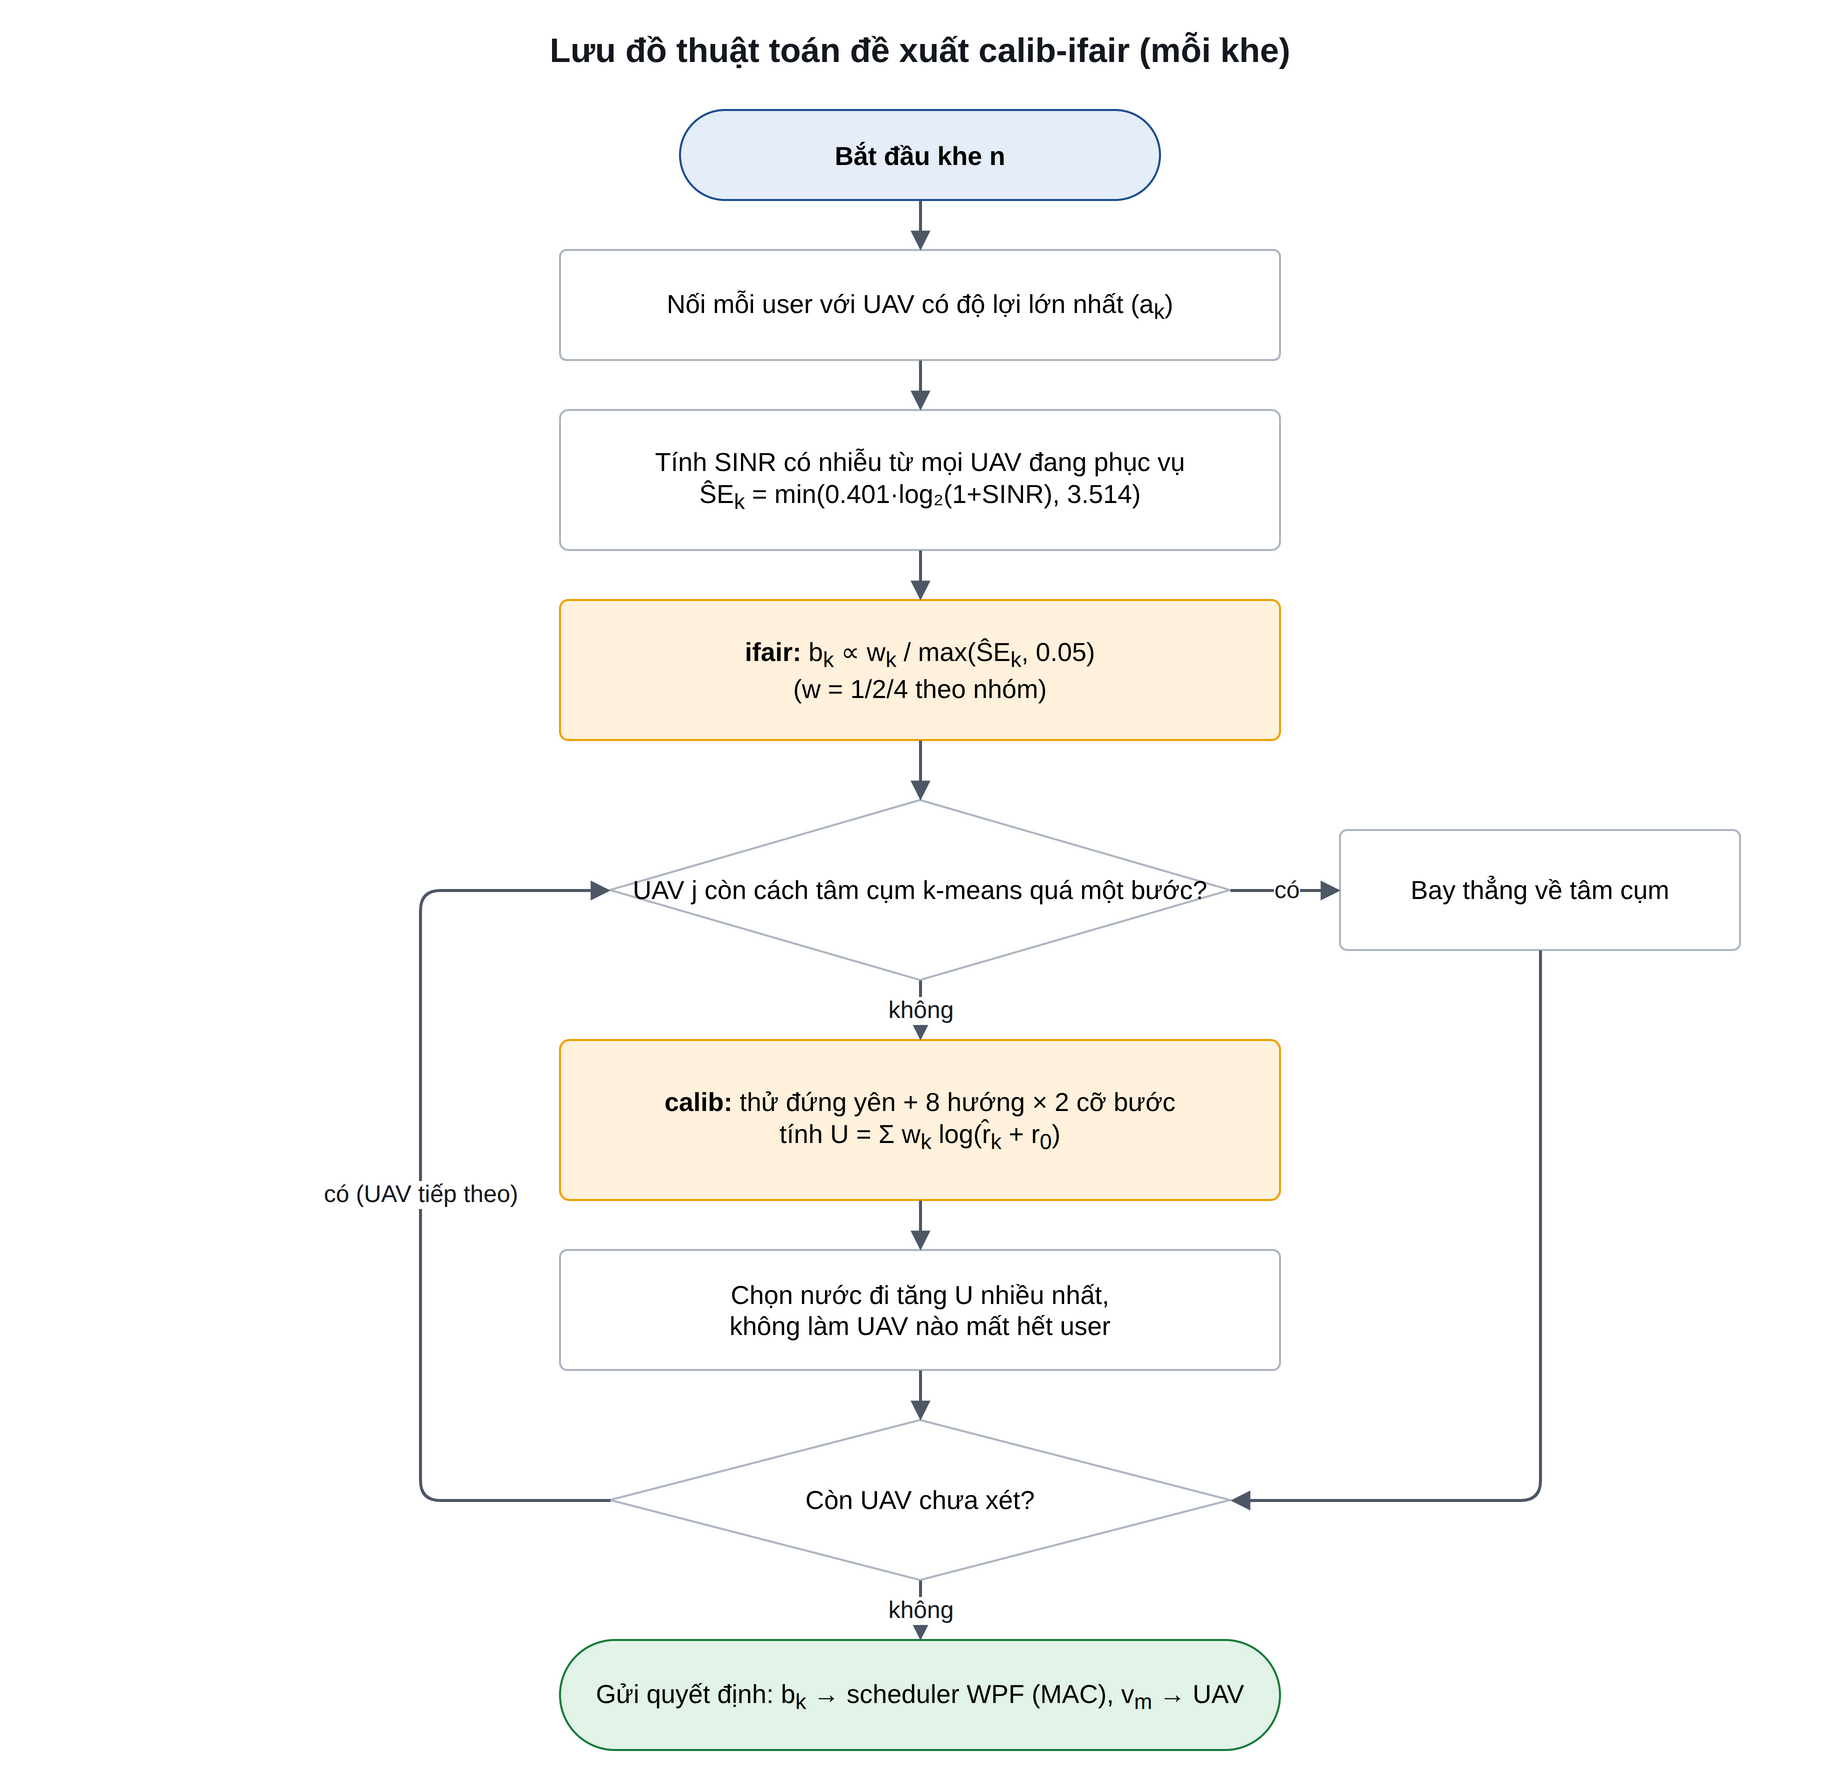
\includegraphics[height=0.80\textheight]{calib_ifair.png}
\end{column}
\begin{column}{0.54\textwidth}
  \small
  \begin{enumerate}
    \setlength{\itemsep}{3pt}
    \item Nối mỗi user với UAV có kênh mạnh nhất.
    \item Tính SINR \hl{có nhiễu} từ mọi UAV đang phục vụ, đổi ra $\SE_k$.
    \item \hl{ifair}: chia băng $b_k \propto w_k / \max(\SE_k, 0.05)$.
    \item Với từng UAV: còn xa tâm cụm k-means thì bay thẳng tới tâm.
    \item Đã tới: thử 17 nước đi, giữ nước làm tiện ích $U$ tăng nhiều nhất, không tắt UAV nào.
    \item Gửi $b_k$ xuống tầng MAC (scheduler WPF), $v_m$ cho UAV.
  \end{enumerate}
  \begin{block}{Thời gian}
    \small
    5.5 ms/khe (3 UAV, 20 user); 13.6 ms/khe (8 UAV, 60 user). Khe dài 250 ms.
  \end{block}
\end{column}
\end{columns}
\end{frame}

% =================================================
% SLIDE 10. KHỐI 1
% =================================================
\begin{frame}{Khối 1: liên kết và SINR có nhiễu}
\begin{columns}[T,onlytextwidth]
\begin{column}{0.52\textwidth}
  \begin{block}{Liên kết}
    \vspace{-2mm}
    \[ a_k = \arg\max_m\ g_{mk}(q_m) \]
    \small User nối UAV có độ lợi kênh lớn nhất.
  \end{block}
  \begin{block}{SINR có nhiễu}
    \vspace{-2mm}
    \[
      \mathrm{SINR}_k = \frac{\mathrm{psd}_{a_k}\, g_{a_k k}}{\sum_{j\ne a_k}\mathrm{psd}_j\, g_{jk} + N_0}
    \]
    \[
      \mathrm{psd}_m = \begin{cases}P_{\max}/B, & \text{UAV } m \text{ có user}\\0, & \text{ngược lại}\end{cases}
    \]
  \end{block}
\end{column}
\begin{column}{0.44\textwidth}
  \begin{block}{Khác baseline ở đâu}
    \small
    \begin{itemize}
      \item Baseline \texttt{maxmin} tính \textbf{SNR không nhiễu}: user ở giữa hai UAV trông như kênh tốt, thật ra bị nhiễu nặng.
      \item calib-ifair tính \hl{SINR có nhiễu}: biết đúng user nào thật sự yếu để bù băng.
      \item UAV không có user thì không phát, nên không gây nhiễu.
    \end{itemize}
  \end{block}
\end{column}
\end{columns}
\end{frame}

% =================================================
% SLIDE 11. KHỐI 2 - CÔNG THỨC
% =================================================
\begin{frame}{Khối 2: chia băng ifair}
\begin{block}{Công thức}
\vspace{-3mm}
\[
b_k = \frac{w_k / \max(\SE_k,\ 0.05)}{\displaystyle\sum_{k':\,a_{k'}=a_k} w_{k'} / \max(\SE_{k'},\ 0.05)}
\quad\Longrightarrow\quad
\hat r_k = \frac{B\,w_k}{\displaystyle\sum_{k':\,a_{k'}=a_k} w_{k'}/\SE_{k'}}
\]
\end{block}
\begin{columns}[T,onlytextwidth]
\begin{column}{0.48\textwidth}
  \begin{block}{Ý nghĩa}
    \small
    \begin{itemize}
      \item Trong một UAV, $\hat r_k / w_k$ bằng nhau: \hl{max-min có trọng số}.
      \item User critical luôn được tốc độ gấp 4 lần user normal cùng UAV, dù kênh xấu hơn.
      \item User kênh xấu (SE nhỏ) được bù nhiều băng hơn.
      \item Sàn 0.05: user gần mất sóng không hút hết băng.
    \end{itemize}
  \end{block}
\end{column}
\begin{column}{0.48\textwidth}
  \begin{block}{Vì sao không dùng nghiệm tổng log}
    \small
    Bài toán con $\max\sum w_k\log(b_k B\,\SE_k)$, $\sum b_k\le1$ có nghiệm $b_k = w_k/\sum w$: băng tỷ lệ với $w$,
    \textbf{không phụ thuộc kênh}, nên user critical ở rìa vẫn chậm.
    ifair cố ý chia để \hl{tốc độ} tỷ lệ với $w$; hàm $U$ chỉ dùng để chọn vị trí UAV ở khối 3.
  \end{block}
\end{column}
\end{columns}
\end{frame}

% =================================================
% SLIDE 12. KHỐI 2 - VÍ DỤ SỐ
% =================================================
\begin{frame}{Khối 2: ví dụ số}
\small Một UAV, $B = 10$ MHz, ba user có hiệu suất phổ khác nhau:
\vspace{2mm}

\begin{tabularx}{\linewidth}{@{}lccXXX@{}}
  \toprule
  \textbf{User} & $w$ & $\SE$ (bit/s/Hz) & \textbf{Chia đều} & \textbf{max-min (không trọng số)} & \textbf{ifair}\\
  \midrule
  normal & 1 & 3.0 & $b=0.33$, \ 10.0 Mbps & $b=0.18$, \ 5.45 Mbps & $b=0.06$, \ \textbf{1.88 Mbps}\\
  important & 2 & 2.0 & $b=0.33$, \ 6.67 Mbps & $b=0.27$, \ 5.45 Mbps & $b=0.19$, \ \textbf{3.75 Mbps}\\
  \textcolor{Bad}{critical} & 4 & 1.0 & $b=0.33$, \ \alert{3.33 Mbps} & $b=0.55$, \ 5.45 Mbps & $b=0.75$, \ \good{7.50 Mbps}\\
  \midrule
  \textbf{Tổng} & & & 20.0 Mbps & 16.4 Mbps & 13.1 Mbps\\
  \bottomrule
\end{tabularx}

\vspace{3mm}
\begin{columns}[T,onlytextwidth]
\begin{column}{0.48\textwidth}
  \begin{block}{Cách tính ifair}
    \scriptsize
    $x_k = w_k/\SE_k = 0.33,\ 1,\ 4$; tổng $5.33$\\
    $b_k = x_k/5.33 = 0.0625,\ 0.1875,\ 0.75$\\
    $r_k = b_k\,B\,\SE_k = 1.88,\ 3.75,\ 7.50$ Mbps $\Rightarrow$ tỷ lệ \hl{1 : 2 : 4}
  \end{block}
\end{column}
\begin{column}{0.48\textwidth}
  \begin{block}{Đọc bảng}
    \scriptsize
    Chia đều: critical (kênh xấu nhất) chậm nhất. max-min: mọi user bằng nhau, critical không được ưu tiên.
    ifair: critical nhanh nhất, đổi lại tổng tốc độ giảm. Đây là đánh đổi có chủ đích, chỉnh được bằng $w$.
  \end{block}
\end{column}
\end{columns}
\end{frame}

% =================================================
% SLIDE 13. KHỐI 3
% =================================================
\begin{frame}{Khối 3: di chuyển calib}
\begin{columns}[T,onlytextwidth]
\begin{column}{0.52\textwidth}
  \begin{block}{Hai pha cho mỗi UAV}
    \small
    \textbf{Tiếp cận:} còn cách tâm cụm k-means $c_j$ hơn $V_{\max}\Delta t$ thì bay thẳng về $c_j$.\\[1mm]
    \textbf{Tinh chỉnh:} thử 17 nước đi, chọn
    \[
      d^\star_j = \arg\max_{d\in\mathcal{D}} U\big(q_1,\dots,q_j+d,\dots,q_M\big)
    \]
    \[
      \mathcal{D} = \{0\}\cup\{s(\cos\tfrac{i\pi}{4},\sin\tfrac{i\pi}{4})\},\ i=0..7,\ s\in\{V_{\max}\Delta t,\tfrac14V_{\max}\Delta t\}
    \]
  \end{block}
  \begin{block}{Quy tắc}
    \scriptsize
    \begin{itemize}
      \item Xét lần lượt từng UAV; UAV sau thấy vị trí mới của UAV trước.
      \item $U$ tính lại có nhiễu, có trần LTE, có trọng số nhóm.
      \item Loại nước đi làm giảm số UAV có user.
    \end{itemize}
  \end{block}
\end{column}
\begin{column}{0.44\textwidth}
  \centering
  \begin{tikzpicture}[scale=1.05]
    \fill[MainBlue!6] (-2.3,-2.3) rectangle (2.3,2.3);
    \foreach \i in {0,...,7} {
      \draw[arr,draw=Accent!80] (0,0) -- ({1.9*cos(45*\i)},{1.9*sin(45*\i)});
      \fill[Accent] ({1.9*cos(45*\i)},{1.9*sin(45*\i)}) circle (2pt);
      \fill[orange] ({0.6*cos(45*\i)},{0.6*sin(45*\i)}) circle (2pt);
    }
    \fill[U0] (0,0) circle (5pt);
    \node[font=\scriptsize,below=3pt] at (0,-0.1) {UAV};
    \node[font=\scriptsize,anchor=west] at (-2.25,2.05) {\textcolor{Accent}{$\bullet$} bước $V_{\max}\Delta t$ = 5 m};
    \node[font=\scriptsize,anchor=west] at (-2.25,-2.05) {\textcolor{orange}{$\bullet$} bước 1.25 m, \ \textcolor{U0}{$\bullet$} đứng yên};
  \end{tikzpicture}

  {\scriptsize 17 ứng viên với $V_{\max}=20$ m/s, $\Delta t=0.25$ s. Mỗi ứng viên tính lại $U$ toàn mạng.}
\end{column}
\end{columns}
\end{frame}

% =================================================
% SLIDE 14. MÃ GIẢ 1
% =================================================
\begin{frame}{Mã giả (1/2): hàm hỗ trợ}
\begin{pseudo}
\kw{Hàm} SE\_DỰ\_ĐOÁN($q$, vị trí user):\\
\> \kw{với mỗi} UAV $m$, user $k$: $g[m,k] \leftarrow$ độ lợi kênh Al-Hourani$(q_m, u_k)$\\
\> $a_k \leftarrow \arg\max_m g[m,k]$ \cm{liên kết}\\
\> $\mathrm{psd}_m \leftarrow P_{\max}/B$ nếu UAV $m$ có user, ngược lại $0$ \cm{UAV trống không phát}\\
\> \kw{với mỗi} user $k$:\\
\>\> $S \leftarrow \mathrm{psd}_{a_k}\, g[a_k,k]$; \quad $I \leftarrow \sum_{j\ne a_k}\mathrm{psd}_j\, g[j,k]$ \cm{nhiễu đồng kênh}\\
\>\> $\mathrm{SINR}_k \leftarrow S/(I+N_0)$\\
\>\> $\SE_k \leftarrow 0$ nếu $\mathrm{SINR}_k < 0.1$, ngược lại $\min(0.401\log_2(1+\mathrm{SINR}_k),\ 3.514)$\\
\> \kw{trả về} $(a, \SE)$\\[2mm]
\kw{Hàm} TIỆN\_ÍCH($q$, vị trí user, $w$):\\
\> $(a,\SE) \leftarrow$ SE\_DỰ\_ĐOÁN($q$, vị trí user)\\
\> \kw{với mỗi} UAV $m$: \ tải$_m \leftarrow \sum_{k:\,a_k=m} w_k/\max(\SE_k, 10^{-3})$\\
\> \kw{với mỗi} user $k$: \ $\hat r_k \leftarrow B\,w_k/\text{tải}_{a_k}$ nếu $\SE_k>0$, ngược lại $0$\\
\> \kw{trả về} $\big(\sum_k w_k\ln(\hat r_k + r_0),\ \text{số UAV có user}\big)$
\end{pseudo}
\end{frame}

% =================================================
% SLIDE 15. MÃ GIẢ 2
% =================================================
\begin{frame}{Mã giả (2/2): một khe của calib-ifair}
\begin{pseudo}
\kw{Thủ tục} CALIB\_IFAIR($q$, vị trí user, nhóm):\\
\> $w_k \leftarrow \{1, 2, 4\}[\text{nhóm}_k]$\\
\> $(a,\SE) \leftarrow$ SE\_DỰ\_ĐOÁN($q$, vị trí user) \cm{khối 1}\\
\> $x_k \leftarrow w_k/\max(\SE_k, 0.05)$; \quad $b_k \leftarrow x_k / \sum_{k':\,a_{k'}=a_k} x_{k'}$; \quad $p_k \leftarrow b_k P_{\max}$ \cm{khối 2: ifair}\\
\> $c \leftarrow$ KMEANS(vị trí user, khởi tạo $= q$); \quad $q' \leftarrow q$ \cm{khối 3: calib}\\
\> \kw{với mỗi} UAV $j = 1..M$:\\
\>\> \kw{nếu} $\|c_j - q'_j\| > V_{\max}\Delta t$: \ $q'_j \leftarrow q'_j + V_{\max}\Delta t\cdot\frac{c_j-q'_j}{\|c_j-q'_j\|}$; \ \kw{tiếp tục} \cm{pha tiếp cận}\\
\>\> $(U^\ast, N^\ast) \leftarrow$ TIỆN\_ÍCH($q'$, vị trí user, $w$); \quad $d^\ast \leftarrow 0$\\
\>\> \kw{với mỗi} $d \in \mathcal{D}\setminus\{0\}$: \cm{16 nước đi}\\
\>\>\> $\tilde q \leftarrow q'$; \ $\tilde q_j \leftarrow \mathrm{clip}(q'_j + d, 0, L)$\\
\>\>\> $(U, N) \leftarrow$ TIỆN\_ÍCH($\tilde q$, vị trí user, $w$)\\
\>\>\> \kw{nếu} $N \ge N^\ast$ \kw{và} $U > U^\ast$: \ $U^\ast \leftarrow U$; \ $d^\ast \leftarrow d$ \cm{không tắt UAV}\\
\>\> $q'_j \leftarrow \mathrm{clip}(q'_j + d^\ast, 0, L)$\\
\> $v \leftarrow (q' - q)/\Delta t$\\
\> \kw{trả về} $(a, b, p, v)$ \cm{$b$ $\rightarrow$ trọng số WPF ở tầng MAC}
\end{pseudo}
\vspace{1mm}
\scriptsize \textbf{Độ phức tạp mỗi khe:} k-means $O(IMK)$, chia băng $O(MK)$, di chuyển $O(17\,M\cdot MK)$.
\end{frame}

% =================================================
% SLIDE 16. ÁP Ở TẦNG MAC VÀ BA TẦNG
% =================================================
\begin{frame}{Áp quyết định ở tầng MAC và kiểm chứng ba tầng}
\begin{columns}[T,onlytextwidth]
\begin{column}{0.40\textwidth}
  \begin{block}{Scheduler Weighted PF}
    \small
    \begin{itemize}
      \item PF mặc định của LTE \alert{tự chia lại} tài nguyên: quyết định $b_k$ của thuật toán mất tác dụng.
      \item Nhóm viết scheduler \hl{WPF} trong NS-3, nhận $b_k$ làm trọng số.
      \item Với WPF, chia băng max-min tăng min throughput 15--21\% (mô hình dự đoán +18\%).
    \end{itemize}
  \end{block}
\end{column}
\begin{column}{0.56\textwidth}
  \centering
  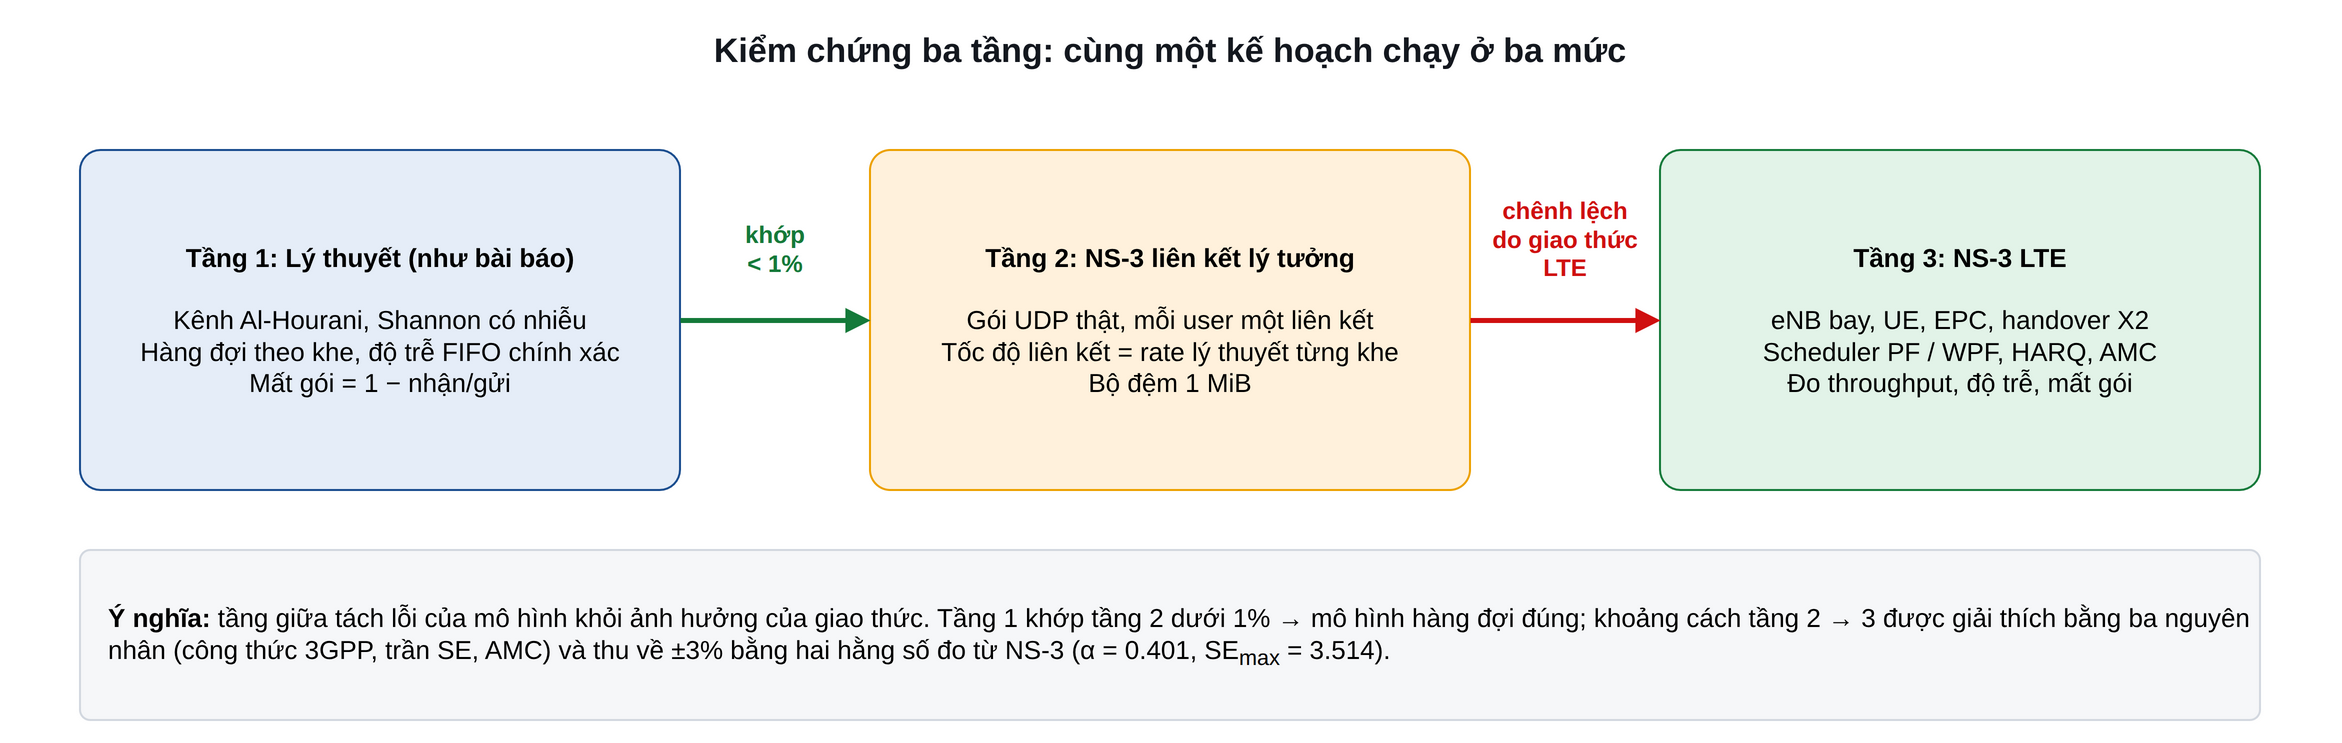
\includegraphics[width=\linewidth]{ba_tang.png}

  \scriptsize Lý thuyết khớp NS-3 liên kết lý tưởng \good{dưới 1\%} (105 run): mô hình đúng ở mức gói tin; chênh lệch còn lại do giao thức LTE.
\end{column}
\end{columns}
\end{frame}

% =================================================
% CÁC BASELINE
% =================================================
\begin{frame}{Các thuật toán tham chiếu (baseline)}
\small
\begin{tabularx}{\linewidth}{@{}lXX@{}}
  \toprule
  \textbf{Thuật toán} & \textbf{Di chuyển UAV} & \textbf{Chia băng trong mỗi UAV}\\
  \midrule
  hover-equal & Đứng yên tại vị trí ban đầu & Chia đều: $b_k = 1/|\mathcal{K}_m|$\\
  kmeans-equal & Bay về tâm cụm user (k-means) & Chia đều\\
  kmeans-maxmin & Bay về tâm cụm & $b_k \propto 1/\log_2(1+\mathrm{SNR}_k)$: tốc độ bằng nhau, SNR \alert{không nhiễu}\\
  kmeans-wmaxmin & Bay về tâm cụm & $b_k \propto w_k/\log_2(1+\mathrm{SNR}_k)$: max-min \hl{có trọng số nhóm}, không nhiễu\\
  \midrule
  calib-ifair-noclass & Như calib-ifair & Như ifair nhưng mọi $w_k = 1$\\
  calib-ifair-shannon & Như calib-ifair, tính $U$ bằng Shannon & Như ifair, $\widehat{SE} = \log_2(1+\mathrm{SINR})$\\
  kmeans-ifair, calib-equal & Bỏ khối di chuyển / bỏ khối chia băng & (bản tách thành phần)\\
  \bottomrule
\end{tabularx}
\vspace{2mm}
\begin{columns}[T,onlytextwidth]
\begin{column}{0.48\textwidth}
  \begin{block}{Vì sao chọn các baseline này}
    \scriptsize
    equal đại diện ``tối đa hiệu quả'', maxmin đại diện ``tối đa công bằng'' -- hai cách phổ biến trong các bài báo UAV-BS.
    wmaxmin là đối thủ \textbf{cùng biết nhóm} để so sánh công bằng.
  \end{block}
\end{column}
\begin{column}{0.48\textwidth}
  \begin{block}{Điều kiện so sánh}
    \scriptsize
    Cùng kịch bản, cùng seed (vị trí user, nhóm), cùng lưu lượng; liên kết theo kênh mạnh nhất; mọi thuật toán chấm bằng cùng chỉ số đo trên NS-3.
  \end{block}
\end{column}
\end{columns}
\end{frame}

% =================================================
% CÀI ĐẶT HỆ THỐNG
% =================================================
\begin{frame}{Cài đặt hệ thống}
\begin{columns}[T,onlytextwidth]
\begin{column}{0.44\textwidth}
  \small
  \begin{tabularx}{\linewidth}{@{}>{\raggedright\arraybackslash}p{0.40\linewidth}>{\raggedright\arraybackslash}X@{}}
    \toprule
    \textbf{Thành phần} & \textbf{Công nghệ}\\
    \midrule
    Mô hình, thuật toán & Python 3.10, NumPy\\
    Mô phỏng mạng & NS-3 3.47, module LTE (LENA), EPC, C++\\
    Scheduler WPF & Viết thêm trong NS-3 (C++)\\
    Điều khiển thời gian thực & asyncio, WebSocket, HTML5 canvas\\
    Hiển thị 3D & Gazebo Harmonic, gz-transport\\
    Kiểm thử & pytest, 42 test\\
    \bottomrule
  \end{tabularx}

  \vspace{2mm}
  \scriptsize Mỗi thí nghiệm lưu kèm cấu hình; chạy lại cho kết quả trùng từng chữ số.
\end{column}
\begin{column}{0.52\textwidth}
  \centering
  \textbf{\small Quy trình đo một thuật toán}
  \vspace{2mm}

  \begin{tikzpicture}[node distance=3.5mm]
    \node[box,text width=5.6cm] (a) {\textbf{1. uavsim chạy thuật toán}\\\scriptsize ra quyết định $a, b, v$ từng khe};
    \node[box,text width=5.6cm,below=of a] (b) {\textbf{2. Ghi kế hoạch}\\\scriptsize uavs.csv (quỹ đạo), users.csv (liên kết, $b_k$)};
    \node[box,text width=5.6cm,below=of b,fill=Accent!12] (c) {\textbf{3. NS-3 phát lại kế hoạch}\\\scriptsize eNB bay theo quỹ đạo, handover X2 theo liên kết, WPF dùng $b_k$, UDP $\lambda$};
    \node[box,text width=5.6cm,below=of c] (d) {\textbf{4. Đo từng user từng khe}\\\scriptsize byte, gói gửi/nhận, độ trễ $\rightarrow$ chỉ số theo nhóm};
    \draw[arr] (a) -- (b); \draw[arr] (b) -- (c); \draw[arr] (c) -- (d);
  \end{tikzpicture}
\end{column}
\end{columns}
\end{frame}

% =================================================
% THÔNG SỐ THÍ NGHIỆM
% =================================================
\begin{frame}{Thông số thí nghiệm}
\begin{columns}[T,onlytextwidth]
\begin{column}{0.48\textwidth}
  \scriptsize
  \begin{tabularx}{\linewidth}{@{}>{\raggedright\arraybackslash}p{0.44\linewidth}>{\raggedright\arraybackslash}X@{}}
    \toprule
    \textbf{Tham số} & \textbf{Giá trị}\\
    \midrule
    Số UAV $M$ / số user $K$ & 3 / 20\\
    Nhóm user & 3 critical, 5 important, 12 normal\\
    Vùng / độ cao UAV & $1000\times1000$ m / 100 m\\
    Phân bố user & theo cụm, đứng yên\\
    Môi trường kênh & đô thị (Al-Hourani: $a=9.61$, $b=0.16$, $\eta=1/20$ dB)\\
    Tần số / băng thông & 2 GHz / 10 MHz (50 RB)\\
    Công suất phát mỗi UAV & 1 W (30 dBm)\\
    Mật độ nhiễu & $-169$ dBm/Hz (noise figure 5 dB)\\
    Vận tốc tối đa & 20 m/s\\
    \bottomrule
  \end{tabularx}
\end{column}
\begin{column}{0.48\textwidth}
  \scriptsize
  \begin{tabularx}{\linewidth}{@{}>{\raggedright\arraybackslash}p{0.44\linewidth}>{\raggedright\arraybackslash}X@{}}
    \toprule
    \textbf{Tham số} & \textbf{Giá trị}\\
    \midrule
    Khe / số khe & 1 s / 60 khe (+0.5 s khởi động)\\
    Lưu lượng mỗi user $\lambda$ & 0.5, 1, 1.5, 2, 2.5, 3, 4 Mbps\\
    Gói UDP / bộ đệm & 1200 byte / 1 MiB mỗi user\\
    Scheduler MAC & WPF (PF cho kmeans-equal)\\
    Trọng số nhóm $w$ & 1 / 2 / 4\\
    $r_{\min}$ theo nhóm & 0.5 / 1 / 2 Mbps\\
    Số seed & 3 (cùng seed cho mọi thuật toán)\\
    Số run NS-3 cho thí nghiệm nhóm & 63 mới + dùng lại run cũ\\
    Tổng số run NS-3 của dự án & khoảng 500\\
    \bottomrule
  \end{tabularx}
\end{column}
\end{columns}
\vspace{2mm}
\scriptsize Dashboard dùng khe 0.25 s để chuyển động mượt; thí nghiệm NS-3 dùng khe 1 s.
\end{frame}

% =================================================
% SLIDE 17. THIẾT LẬP THÍ NGHIỆM
% =================================================
\begin{frame}{Thiết lập thí nghiệm}
\begin{columns}[T,onlytextwidth]
\begin{column}{0.36\textwidth}
  \begin{block}{NS-3 3.47 LTE}
    \scriptsize
    \begin{itemize}
      \item eNB bay theo kế hoạch, UE, EPC, handover X2.
      \item UDP CBR, 7 mức tải 0.5--4 Mbps/user.
      \item 3 UAV, 20 user (3 critical, 5 important, 12 normal), 60 khe, 3 seed.
      \item Đo từng user từng khe: byte, gói, độ trễ.
    \end{itemize}
  \end{block}
  \begin{block}{Chỉ số}
    \scriptsize
    Throughput tổng; min throughput và tỷ lệ đạt QoS theo nhóm; độ trễ theo nhóm; mất gói $1 - \frac{\text{nhận}}{\text{gửi}}$.
    Đạt QoS: $\mathrm{thr} \ge \min(r_{\min,c}, 0.9\lambda)$.
  \end{block}
\end{column}
\begin{column}{0.60\textwidth}
  \scriptsize
  \begin{tabularx}{\linewidth}{@{}lXlc@{}}
    \toprule
    \textbf{Thuật toán} & \textbf{Mục tiêu} & \textbf{Tốc độ dùng} & \textbf{Biết nhóm}\\
    \midrule
    kmeans-equal & gần $\max\sum r$ & -- & không\\
    kmeans-maxmin & $\max\min r$ & Shannon, bỏ nhiễu & không\\
    kmeans-wmaxmin & $\max\min r/w$ & Shannon, bỏ nhiễu & \textbf{có}\\
    calib-ifair-noclass & $\sum\log r$ & LTE, có nhiễu & không\\
    calib-ifair-shannon & $\sum w\log r$ & Shannon, có nhiễu & có\\
    \hl{calib-ifair} & \hl{$\sum w\log r$} & \hl{LTE, có nhiễu} & \hl{có}\\
    \bottomrule
  \end{tabularx}

  \vspace{2mm}
  kmeans-wmaxmin là baseline \hl{cùng biết nhóm}: so sánh trên cùng thông tin, chỉ khác phương pháp.
  Hai bản noclass, shannon cùng thuật toán, bỏ một yếu tố để tách nguồn gốc lợi ích.
\end{column}
\end{columns}
\end{frame}

% =================================================
% SLIDE 18. KẾT QUẢ - HÌNH
% =================================================
\begin{frame}{Kết quả trên NS-3 LTE}
\centering
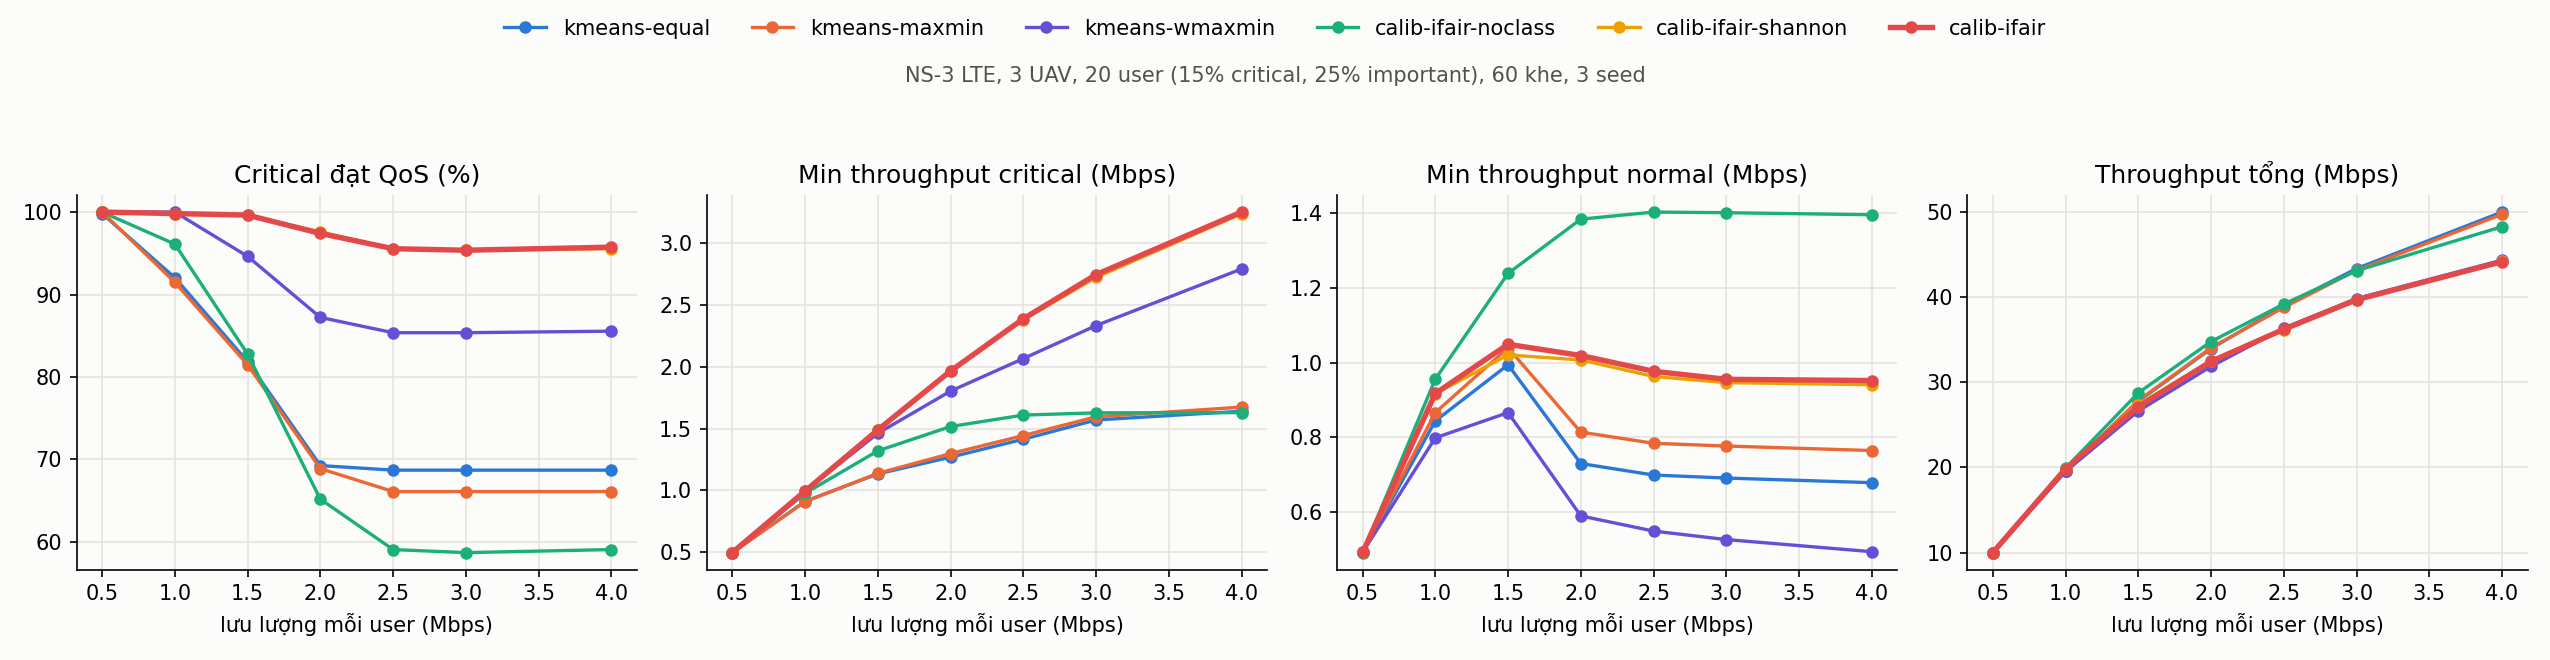
\includegraphics[width=\linewidth]{classes.png}

\small
calib-ifair (đỏ đậm) giữ \good{95--100\%} user critical đạt QoS ở mọi mức tải; baseline không biết nhóm tụt xuống 59--69\%,
max-min có trọng số (tím) dừng ở 86--87\%. Đổi lại throughput tổng ở tải cao thấp hơn baseline không biết nhóm.
\end{frame}

% =================================================
% SLIDE 19. KẾT QUẢ - BẢNG
% =================================================
\begin{frame}{So sánh chi tiết (trung bình 3 seed)}
\small
\begin{tabularx}{\linewidth}{@{}clXXXX@{}}
  \toprule
  \textbf{Mbps/user} & \textbf{Chỉ số} & \textbf{kmeans-equal} & \textbf{kmeans-maxmin} & \textbf{kmeans-wmaxmin} & \textbf{calib-ifair}\\
  \midrule
  2 & Critical đạt QoS & 69\% & 69\% & 87\% & \good{97\%}\\
  2 & Min throughput critical & 1.27 & 1.30 & 1.80 & \good{1.97 Mbps}\\
  2 & Độ trễ critical & 1084 & 1328 & 252 & \good{41 ms}\\
  2 & Min throughput normal & 0.73 & 0.81 & 0.59 & \good{1.02 Mbps}\\
  2 & Throughput tổng & \textbf{33.9} & \textbf{34.0} & 31.8 & 32.4 Mbps\\
  \midrule
  4 & Critical đạt QoS & 69\% & 66\% & 86\% & \good{96\%}\\
  4 & Min throughput critical & 1.64 & 1.67 & 2.79 & \good{3.25 Mbps}\\
  4 & Độ trễ critical & 2062 & 2334 & \textbf{652} & 720 ms\\
  4 & Min throughput normal & 0.68 & 0.76 & 0.49 & \good{0.95 Mbps}\\
  4 & Throughput tổng & \textbf{49.9} & \textbf{49.7} & 44.3 & 44.1 Mbps\\
  4 & Mất gói & \textbf{37.6\%} & 37.9\% & 44.6\% & 44.8\%\\
  \bottomrule
\end{tabularx}
\vspace{2mm}

\scriptsize Ở 1 Mbps/user (tải vừa), calib-ifair tốt hơn ở mọi chỉ số: critical 100\% đạt QoS, độ trễ critical 208 $\rightarrow$ 6 ms, mất gói 2.2\% $\rightarrow$ 0.8\%.
\end{frame}

% =================================================
% SLIDE 20. LỢI ÍCH ĐẾN TỪ ĐÂU
% =================================================
\begin{frame}{Lợi ích đến từ đâu}
\begin{columns}[T,onlytextwidth]
\begin{column}{0.52\textwidth}
  \small
  \begin{tabularx}{\linewidth}{@{}Xc@{}}
    \toprule
    \textbf{So sánh (4 Mbps/user)} & \textbf{Kết quả}\\
    \midrule
    Bỏ trọng số nhóm (noclass) & critical QoS 96\% $\rightarrow$ \alert{59\%}\\
    Bỏ tính nhiễu + tinh chỉnh (wmaxmin) & 96\% $\rightarrow$ 86\%, normal $\div$2\\
    Bỏ khối chia băng (calib-equal)* & min 1.37 $\rightarrow$ 0.75 Mbps\\
    Bỏ khối di chuyển (kmeans-ifair)* & tổng 48.2 $\rightarrow$ 46.1 Mbps\\
    Shannon thay LTE (shannon) & \textbf{như nhau} (1--2\%)\\
    PF thay WPF ở MAC & chia băng mất tác dụng\\
    \bottomrule
  \end{tabularx}

  \scriptsize * thí nghiệm không chia nhóm (mọi $w=1$).
\end{column}
\begin{column}{0.44\textwidth}
  \begin{block}{Kết luận}
    \small
    Lợi ích đến từ: \hl{trọng số nhóm}, \hl{tính nhiễu khi chia băng}, \hl{tinh chỉnh vị trí} và \hl{áp ở tầng MAC}.
  \end{block}
  \begin{block}{Phát hiện trung thực}
    \small
    Đường cong LTE hiệu chỉnh giúp \textbf{dự đoán} số đo NS-3 ($\pm$2\%) nhưng \textbf{không} làm thuật toán tốt hơn:
    thứ tự ưu tiên giữa các user gần như giống nhau dù dùng Shannon hay LTE.
  \end{block}
\end{column}
\end{columns}
\end{frame}

% =================================================
% SLIDE 21. HỆ THỐNG THỜI GIAN THỰC
% =================================================
\begin{frame}{Trạm điều khiển thời gian thực}
\begin{columns}[T,onlytextwidth]
\begin{column}{0.62\textwidth}
  \centering
  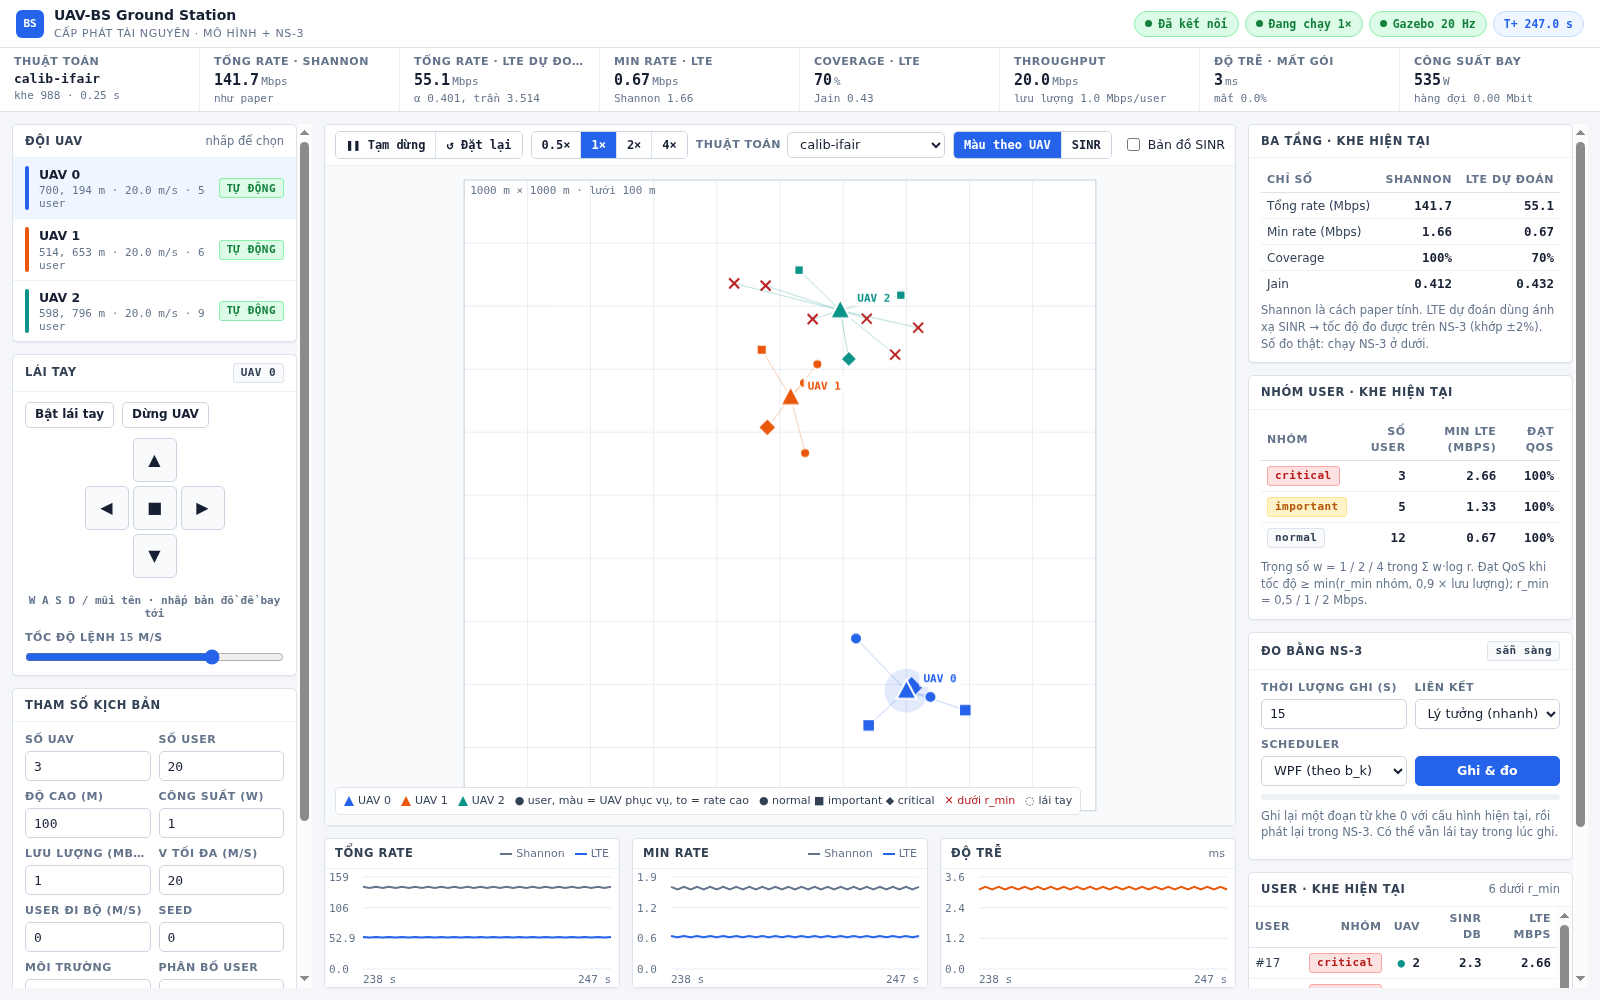
\includegraphics[width=\linewidth]{dashboard.png}

  {\scriptsize Dashboard web chạy calib-ifair: bảng nhóm user cho thấy 100\% critical đạt QoS.}
\end{column}
\begin{column}{0.34\textwidth}
  \small
  \begin{itemize}
    \setlength{\itemsep}{3pt}
    \item Khe 0.25 s, web vẽ 60 Hz, Gazebo 20 Hz.
    \item Lái tay UAV, nhấp bản đồ để bay tới.
    \item Đổi 13 tham số khi đang chạy, kể cả tỷ lệ nhóm.
    \item \textbf{Ghi \& đo}: chạy NS-3 ngay từ web.
    \item Gazebo: áo màu UAV phục vụ, vòng vàng important, vòng đỏ critical.
  \end{itemize}
  \vspace{2mm}
  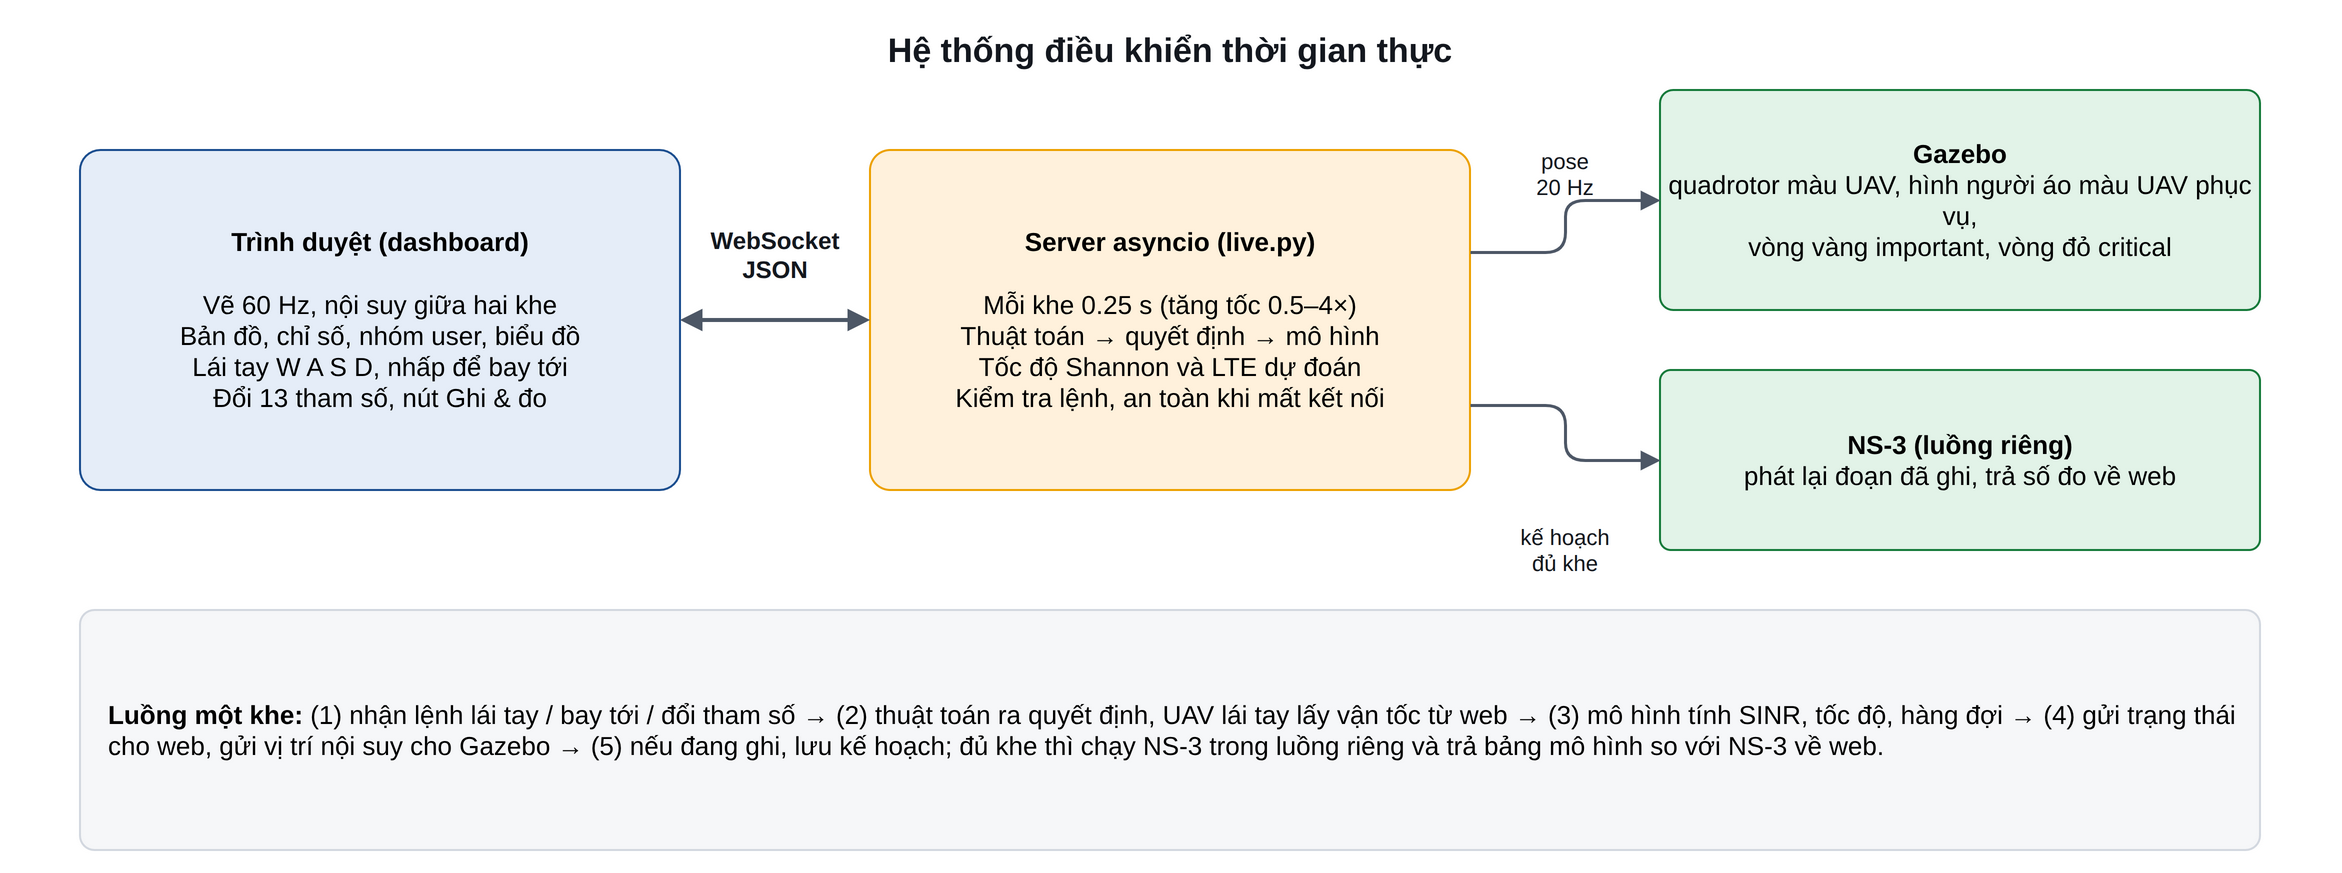
\includegraphics[width=\linewidth]{thoi_gian_thuc.png}
\end{column}
\end{columns}
\end{frame}

% =================================================
% SLIDE 22. ĐÁNH ĐỔI VÀ HẠN CHẾ
% =================================================
\begin{frame}{Đánh đổi và hạn chế}
\begin{columns}[T,onlytextwidth]
\begin{column}{0.48\textwidth}
  \begin{block}{Đánh đổi có chủ đích}
    \small
    \begin{itemize}
      \item Throughput tổng ở tải cao thấp hơn baseline không biết nhóm khoảng 11\%; mất gói cao hơn.
      \item Nhóm normal chịu độ trễ cao hơn, nhưng min throughput vẫn cao hơn mọi baseline.
      \item Mức đánh đổi chỉnh được bằng trọng số $w$.
    \end{itemize}
  \end{block}
\end{column}
\begin{column}{0.48\textwidth}
  \begin{block}{Hạn chế}
    \small
    \begin{itemize}
      \item Heuristic tham lam, tìm cục bộ: không đảm bảo tối ưu toàn cục.
      \item $r_{\min}$ nhóm chưa là ràng buộc cứng.
      \item Công suất, độ cao không tối ưu.
      \item Một cấu hình, 3 seed; chưa có baseline tối ưu lồi (BCD + SCA).
      \item NS-3 phát lại kế hoạch, chưa vòng kín; SISO, không fading.
    \end{itemize}
  \end{block}
\end{column}
\end{columns}
\end{frame}

% =================================================
% SLIDE 23. KẾT LUẬN
% =================================================
\begin{frame}{Kết luận}
\begin{columns}[T,onlytextwidth]
\begin{column}{0.58\textwidth}
  \small
  \renewcommand{\arraystretch}{1.15}
  \begin{tabularx}{\linewidth}{@{}Xl@{}}
    \toprule
    \textbf{Kết luận} & \textbf{Trên NS-3 LTE}\\
    \midrule
    Mô hình hàng đợi đúng ở mức gói tin & \good{Đúng}, sai số $<$1\%\\
    Giá trị tuyệt đối theo Shannon & \alert{Lạc quan}, 25--40\%\\
    Chia băng chỉ có tác dụng khi áp ở MAC & \good{Đúng} (WPF)\\
    calib-ifair ưu tiên được critical & \good{96--97\%} đạt QoS\\
    Hơn max-min có trọng số cùng biết nhóm & \good{Đúng}, tổng như nhau\\
    LTE hiệu chỉnh tốt hơn Shannon khi quyết định & \alert{Không}\\
    \bottomrule
  \end{tabularx}
\end{column}
\begin{column}{0.38\textwidth}
  \begin{block}{Hướng phát triển}
    \small
    \begin{itemize}
      \item Ràng buộc $r_{\min}$ cứng cho critical.
      \item Baseline tối ưu lồi có trọng số.
      \item Mở rộng số UAV, môi trường, từ 20 seed.
      \item Học tăng cường; PX4 SITL.
    \end{itemize}
  \end{block}
\end{column}
\end{columns}

\vspace{2mm}
\begin{beamercolorbox}[sep=2mm,rounded=true]{block title}
  \small
  calib-ifair: heuristic cải tiến, \textbf{ưu tiên người dùng critical mà không bỏ rơi các nhóm khác}, kiểm chứng ở mức gói tin bằng NS-3 LTE.
\end{beamercolorbox}
\end{frame}

% =================================================
% SLIDE 24. TÀI LIỆU THAM KHẢO
% =================================================
\begin{frame}{Tài liệu tham khảo}
\scriptsize
\begin{enumerate}
  \setlength{\itemsep}{5pt}
  \item A. Al-Hourani, S. Kandeepan, S. Lardner, ``Optimal LAP Altitude for Maximum Coverage,'' \emph{IEEE Wireless Communications Letters}, vol. 3, no. 6, 2014.
  \item Q. Wu, Y. Zeng, R. Zhang, ``Joint Trajectory and Communication Design for Multi-UAV Enabled Wireless Networks,'' \emph{IEEE Trans. Wireless Communications}, vol. 17, no. 3, 2018.
  \item Y. Zeng, J. Xu, R. Zhang, ``Energy Minimization for Wireless Communication With Rotary-Wing UAV,'' \emph{IEEE Trans. Wireless Communications}, vol. 18, no. 4, 2019.
  \item R. Jain, D. Chiu, W. Hawe, ``A Quantitative Measure of Fairness and Discrimination for Resource Allocation in Shared Computer Systems,'' DEC TR-301, 1984.
  \item 3GPP TR 36.942, ``E-UTRA Radio Frequency (RF) system scenarios,'' Phụ lục A.1.
  \item ns-3 Model Library, LTE Module (LENA), phiên bản 3.47. \url{https://www.nsnam.org}
  \item Gazebo Sim (Harmonic) documentation, Open Robotics. \url{https://gazebosim.org}
\end{enumerate}
\end{frame}

\begin{frame}[plain]
\vfill
\centering
{\fontsize{24}{30}\selectfont\bfseries\color{MainBlue} Cảm ơn thầy cô và các bạn đã lắng nghe!\par}
\vspace{4mm}
{\large\color{black!60} Hỏi đáp\par}
\vfill
\end{frame}

\end{document}
